\documentclass[11pt, letterpaper]{article}
\usepackage{mobi-lectura}

\title{El Teorema del Límite Central}
\author{Alejandra Tabares Pozos}
\date{}

\begin{document}

\maketitle
\thispagestyle{empty}
\setcounter{page}{0}


\pagenumbering{arabic}

%========================================================================================
%   PÁGINA 1: EL PROBLEMA FUNDAMENTAL DEL ANÁLISIS DE SIMULACIÓN
%========================================================================================
\section{Introducción}

Un modelo de simulación es, en esencia, un generador de números aleatorios estructurado. Las entradas del modelo (tiempos entre llegadas, tiempos de servicio, probabilidades de falla) son estocásticas, lo que implica inevitablemente que las salidas del modelo (productividad, tiempo de espera, utilización de recursos) también son estocásticas.

Esto nos presenta un desafío fundamental. Si ejecutamos una simulación de un banco durante un día y obtenemos un tiempo de espera promedio de 5.3 minutos, ¿qué significa este número? Si la volvemos a ejecutar con un conjunto diferente de números aleatorios, podríamos obtener 4.8 minutos. Una tercera ejecución podría arrojar 5.9 minutos. Ninguno de estos valores es la respuesta verdadera; son simplemente realizaciones puntuales de una variable aleatoria.

El objetivo del análisis de simulación no es generar un único número, sino realizar una \textbf{inferencia estadística} sobre el rendimiento en un periodo de tiempo del sistema que estamos estudiando. Necesitamos estimar una media de rendimiento y, lo que es más importante, cuantificar la incertidumbre de esa estimación.

Para lograr esto, no realizamos una única y larga ejecución de la simulación. En su lugar, llevamos a cabo múltiples ejecuciones independientes, llamadas \textbf{réplicas}. Cada réplica es un experimento estadístico independiente que produce una observación de la métrica de rendimiento que nos interesa. Si $Y_i$ es el tiempo de espera promedio observado en la réplica $i$, después de $n$ réplicas, tendremos un conjunto de observaciones $\{Y_1, Y_2, \dots, Y_n\}$.

La pregunta central es: ¿qué podemos decir sobre la verdadera media del tiempo de espera, $\mu = E[Y]$, basándonos en esta muestra de réplicas? La respuesta la proporciona una de las piedras angulares de la estadística: el Teorema Central del Límite.

\newpage
%========================================================================================
%   PÁGINA 2: EL TEOREMA DEL LÍMITE CENTRAL
%========================================================================================
\section{El Teorema Central del Límite (TCL)}

El Teorema del Límite Central es uno de los resultados más notables de la teoría de la probabilidad. Su poder radica en que nos dice algo profundo sobre la distribución de la media de una muestra, independientemente de la forma de la distribución original de la que se extrajo la muestra.

\begin{teorema}[TCL]
Sean $Y_1, Y_2, \dots, Y_n$ variables aleatorias independientes e idénticamente distribuidas (i.i.d.) con una media finita $\mu$ y una varianza finita $\sigma^2$. Sea $\bar{Y}_n = \frac{1}{n}\sum_{i=1}^{n} Y_i$ la media muestral. Entonces, para un $n$ suficientemente grande, la distribución de $\bar{Y}_n$ se aproxima a una distribución Normal con media $\mu$ y varianza $\sigma^2/n$.
\begin{equation}
\bar{Y}_n \approx N\left(\mu, \frac{\sigma^2}{n}\right)
\end{equation}
\end{teorema}

\subsection{Interpretación del Teorema en el Contexto de la Simulación}
Analicemos las condiciones y conclusiones del TLC en nuestro contexto:
\begin{itemize}
    \item \textbf{Variables i.i.d. ($Y_i$):} Cada $Y_i$ es el resultado de una réplica de nuestra simulación (p. ej., el tiempo de espera promedio de la réplica $i$). Para que sean i.i.d., cada réplica debe ejecutarse con una secuencia de números aleatorios independiente (lo que se logra usando diferentes semillas para el generador de números aleatorios). Esta es una práctica estándar en el análisis de simulación.
    
    \item \textbf{Media $\mu$ y Varianza $\sigma^2$ finitas:} Esta es una condición técnica que casi siempre se cumple en los modelos de simulación del mundo real.
    
    \item \textbf{La distribución de $\bar{Y}_n$:} Esta es la distribución de la media de todas nuestras réplicas. El TLC no dice nada sobre la distribución de los $Y_i$ individuales. El tiempo de espera promedio de una sola réplica puede provenir de una distribución muy extraña y sesgada.
    
    \item \textbf{La conclusión monumental:} A pesar de que no conocemos la forma de la distribución de los $Y_i$, el TLC nos garantiza que la distribución de la media muestral $\bar{Y}_n$ será aproximadamente Normal.
\end{itemize}

Esta garantía es la clave que abre la puerta a todo el arsenal de la estadística inferencial clásica, que se basa en gran medida en el supuesto de normalidad.

\newpage
%========================================================================================
%   PÁGINA 3: DEMOSTRACIÓN VISUAL DEL TEOREMA DEL LÍMITE CENTRAL
%========================================================================================
\section{Demostración Visual del TLC con Código}
La afirmación del TLC puede parecer abstracta. La mejor manera de internalizarla es viéndola en acción. Vamos a usar un ejemplo extremo: la tirada de un dado de seis caras. La distribución de una sola tirada es una distribución Uniforme Discreta, que es lo más alejada posible de una distribución Normal.

El siguiente código simula la toma de la media de $n$ tiradas de un dado y grafica la distribución de esta media. Repetiremos el experimento para diferentes valores de $n$.


% En el documento:
\begin{figure}[htbp]
  \centering
  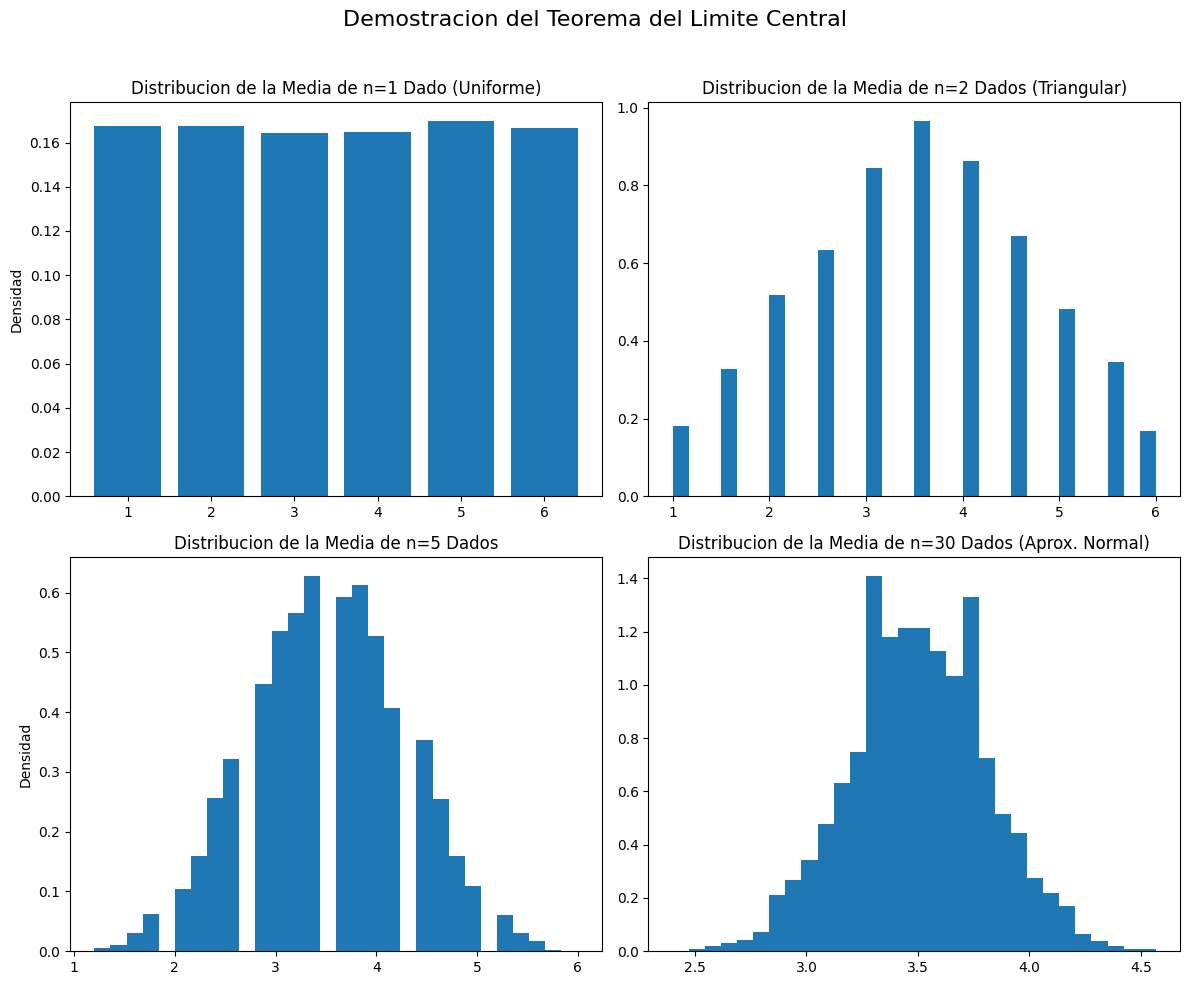
\includegraphics[width=0.8\textwidth]{TCL.png}
  \caption{Ejemplo: TCL}
  \label{fig:mi-imagen}
\end{figure}


Al ejecutar este código, se observa un fenómeno extraordinario: la distribución de las medias muestrales, que comienza siendo perfectamente plana (uniforme) para n=1, se transforma progresivamente en una curva de campana casi perfecta para n=30. Esto sucede a pesar de que la fuente original de aleatoriedad nunca cambia.


%========================================================================================
%   PÁGINA 4: APLICACIÓN PRIMARIA: CONSTRUCCIÓN DE INTERVALOS DE CONFIANZA
%========================================================================================
\section{Uso del resultado TCL: Fundamento de los Intervalos de Confianza}
El resultado más importante del TLC en la simulación es que nos permite construir \textbf{intervalos de confianza} para la media de rendimiento de un sistema. Un intervalo de confianza es un rango de valores que, con un cierto nivel de confianza, contiene el verdadero valor de la media $\mu$.

Dado que el TLC nos dice que $\bar{Y}_n \approx N(\mu, \sigma^2/n)$, podemos estandarizar esta variable:
\[
Z = \frac{\bar{Y}_n - \mu}{\sigma / \sqrt{n}} \approx N(0, 1)
\]
A partir de la distribución Normal estándar, sabemos que para un nivel de confianza de $1-\alpha$, el valor de $Z$ estará entre $-z_{\alpha/2}$ y $z_{\alpha/2}$. Por ejemplo, para un 95\% de confianza, $\alpha=0.05$ y $z_{0.025} = 1.96$.
\[
P\left(-z_{\alpha/2} \le \frac{\bar{Y}_n - \mu}{\sigma / \sqrt{n}} \le z_{\alpha/2}\right) \approx 1-\alpha
\]
Reordenando algebraicamente esta expresión para aislar $\mu$, obtenemos el intervalo de confianza:
\[
\bar{Y}_n - z_{\alpha/2} \frac{\sigma}{\sqrt{n}} \le \mu \le \bar{Y}_n + z_{\alpha/2} \frac{\sigma}{\sqrt{n}}
\]
En la práctica, no conocemos la verdadera desviación estándar de la población, $\sigma$. La reemplazamos por la desviación estándar de nuestra muestra de réplicas, $S$:
\[
S = \sqrt{\frac{1}{n-1}\sum_{i=1}^{n} (Y_i - \bar{Y}_n)^2}
\]
El intervalo de confianza final para la media $\mu$ es:
\begin{equation}
\bar{Y}_n \pm z_{\alpha/2} \frac{S}{\sqrt{n}}
\end{equation}
(Nota: Para $n$ pequeño, típicamente $n < 30$, se debería usar un valor de la distribución t de Student en lugar de $z$, pero para el número de réplicas que se suelen ejecutar en simulación, la aproximación con $z$ es casi siempre adecuada).

Este intervalo es la respuesta final de un estudio de simulación. En lugar de decir el tiempo de espera es 5.3 minutos, decimos: Estamos 95\% seguros de que el verdadero tiempo de espera promedio está entre [4.9, 5.7] minutos. Esta es una afirmación estadísticamente defendible y mucho más valiosa para la toma de decisiones.

\newpage
%========================================================================================
%   PÁGINA 5: EJEMPLO DE CÓDIGO: CÁLCULO DE UN INTERVALO DE CONFIANZA
%========================================================================================
\section{Ejemplo Práctico: Intervalo de Confianza para una Simulación}
Vamos a aplicar este conocimiento. Utilizaremos una función que simula una réplica de un sistema de colas M/M/1 y devuelve el tiempo de espera promedio en la cola. Luego, ejecutaremos múltiples réplicas y construiremos un intervalo de confianza del 95\% para la verdadera media del tiempo de espera.




%===========================
% Diagramas finales (TikZ)
%===========================
% Requiere en el preámbulo:
% \usepackage{graphicx}
% \usepackage{tikz}
% \usetikzlibrary{arrows.meta,positioning,calc,shapes.geometric}

%======================
% FIGURA 1: Mapa A..H
%======================
\begin{figure}[H]
\centering
\resizebox{\linewidth}{!}{%
\begin{tikzpicture}[
  font=\footnotesize,
  box/.style={draw, rounded corners=2mm, align=left, inner sep=6pt},
  hbox/.style={box, text width=5.4cm},
  rbox/.style={box, text width=6.4cm},
  arrow/.style={-Latex, thick},
  node distance=7mm and 18mm
]

% Columna izquierda (Monte Carlo / inferencia)
\node[hbox] (A) {\textbf{A\;\;Fuentes aleatorias}\\[-1mm]
$\Delta A\sim \mathrm{Exp}(\lambda)$,\;\; $S\sim \mathrm{Exp}(\mu)$};

\node[hbox, below=of A] (G) {\textbf{G\;\;Diseño Monte Carlo}\\[-1mm]
$R$ réplicas (semillas)\\
$\Rightarrow$ independencia / reproducibilidad};

\node[hbox, below=of G] (H) {\textbf{H\;\;Inferencia (IC)}\\[-1mm]
$\bar W=\frac1R\sum_{r=1}^R W^{(r)}$\\
$SE=S/\sqrt{R}$\\
IC $\approx \bar W \pm z_{\alpha/2}\,SE$};

% Columna derecha (una réplica / DES)
\node[rbox, right=of A] (B) {\textbf{B\;\;Una réplica (M/M/1)}\\[-1mm]
Entrada: $(\lambda,\mu)$, \texttt{max\_clientes}\\
Salida: $W^{(r)}$ (promedio de esperas)};

\node[rbox, below=of B] (C) {\textbf{C\;\;Estado del sistema}\\[-1mm]
Reloj $t$; contadores $N_A,N_D$\\
Registro de llegadas $t^{(i)}_{\text{arr}}$\\
Lista de esperas $\{W_i\}$};

\node[rbox, below=of C] (D) {\textbf{D\;\;Agenda mínima de eventos}\\[-1mm]
$T_A \leftarrow t+\Delta A$\\
$T_D \leftarrow \infty$ (servidor libre)};

\node[rbox, below=of D] (E) {\textbf{E\;\;Bucle DES (evento más próximo)}\\[-1mm]
\begin{tabular}{@{}l@{}}
si $T_A<T_D$: procesar \textit{llegada}, (re)programar $T_A$, y si\\
\hspace*{2mm} servidor libre entonces programar $T_D=t+S$;\\
si $T_D\le T_A$: procesar \textit{salida} y si cola no vacía\\
\hspace*{2mm} programar el siguiente $T_D=t+S$;\\
parar cuando $N_D=\texttt{max\_clientes}$.
\end{tabular}};

\node[rbox, below=of E] (F) {\textbf{F\;\;Estadística por réplica}\\[-1mm]
$W^{(r)}=\frac{1}{N_D}\sum_{i=1}^{N_D} W_i$};

% Conexiones
\draw[arrow] (A) -- (G);
\draw[arrow] (G) -- (H);

\draw[arrow] (A.east) -- (B.west);
\draw[arrow] (B) -- (C);
\draw[arrow] (C) -- (D);
\draw[arrow] (D) -- (E);
\draw[arrow] (E) -- (F);

% La réplica alimenta el Monte Carlo
\draw[arrow] (F.west) .. controls +(-2.0,0.0) and +(2.2,0.0) .. (G.east);

\end{tikzpicture}%
}
\caption{Mapa bloque de código $\leftrightarrow$ concepto de simulación: dentro de cada réplica se ejecuta DES y fuera se hace inferencia Monte Carlo con réplicas.}
\end{figure}

%======================
% FIGURA 2: Flujo DES
%======================
\begin{figure}[H]
\centering
\resizebox{\linewidth}{!}{%
\begin{tikzpicture}[
  font=\small,
  proc/.style={draw, rounded corners=2mm, align=left, inner sep=6pt, text width=11.8cm},
  box/.style={draw, rounded corners=2mm, align=left, inner sep=6pt, text width=6.2cm},
  decision/.style={draw, diamond, aspect=2.2, align=center, inner sep=1pt},
  arrow/.style={-Latex, thick},
  node distance=8mm and 16mm
]

\node[proc] (S0) {\textbf{Estado en tiempo $t$}\\
Agenda: $T_A$ (próxima llegada), $T_D$ (próxima salida)};

\node[decision, below=of S0] (D0) {$T_A<T_D$?};

\node[box, below left=of D0] (L) {\textbf{Llegada}\\
$t\leftarrow T_A,\;\; N_A\leftarrow N_A+1$\\
Registrar $t^{(N_A)}_{\text{arr}}=t$\\
Si servidor libre ($N_A-N_D=1$):\\
\hspace*{2mm} $S\sim\mathrm{Exp}(\mu)$,\;\; $T_D\leftarrow t+S$,\;\; $W_{N_A}=0$\\
Programar llegada: $\Delta A\sim\mathrm{Exp}(\lambda)$,\;\; $T_A\leftarrow t+\Delta A$};

\node[box, below right=of D0] (R) {\textbf{Salida}\\
$t\leftarrow T_D,\;\; N_D\leftarrow N_D+1$\\
Si cola no vacía ($N_A>N_D$):\\
\hspace*{2mm} $S\sim\mathrm{Exp}(\mu)$,\;\; $T_D\leftarrow t+S$\\
\hspace*{2mm} $W_{N_D+1}=t-t^{(N_D+1)}_{\text{arr}}$\\
Si cola vacía: $T_D\leftarrow \infty$};

% Decisión de paro colocada debajo de ambas ramas (evita cruces)
\coordinate (midLR) at ($(L.south)!0.5!(R.south)$);
\node[decision, below=10mm of midLR] (StopQ) {$N_D=\texttt{max\_clientes}$?};

\node[proc, below=of StopQ] (Out) {\textbf{Salida de la réplica}\\
Retornar $W^{(r)}=\frac{1}{N_D}\sum_{i=1}^{N_D} W_i$};

% Coordenadas para el lazo (misma x en todo el lazo: sin diagonales)
\coordinate (loopXStop) at ([xshift=-14mm]StopQ.west);
\coordinate (loopXS0)   at ([xshift=-14mm]S0.west);

% Flechas
\draw[arrow] (S0) -- (D0);
\draw[arrow] (D0) -- node[left]{\footnotesize sí} (L);
\draw[arrow] (D0) -- node[right]{\footnotesize no} (R);

\draw[arrow] (L.south) -- ++(0,-5mm) -| (StopQ.west);
\draw[arrow] (R.south) -- ++(0,-5mm) -| (StopQ.east);

\draw[arrow] (StopQ) -- node[right]{\footnotesize sí} (Out);

\draw[arrow] (StopQ.west) -- node[above]{\footnotesize no} (loopXStop)
            |- (loopXS0) -- (S0.west);

\end{tikzpicture}%
}
\caption{Flujo DES: cada iteración avanza el reloj al evento más próximo y actualiza la agenda; se repite hasta completar \texttt{max\_clientes}.}
\end{figure}

%========================================================================================
%   PÁGINA 6: CONSIDERACIONES IMPORTANTES Y ERRORES COMUNES
%========================================================================================
\newpage
\section{Consideraciones Prácticas y Errores Comunes}
El TLC es una herramienta robusta, pero su aplicación incorrecta puede llevar a conclusiones erróneas.

\subsection{La Condición de Independencia es Inviolable}
El requisito de que las observaciones $Y_i$ sean independientes es el más crítico. Si, por ejemplo, un analista comete el error de usar la misma semilla para el generador de números aleatorios en cada réplica, obtendrá exactamente el mismo resultado $n$ veces. En este caso, $S=0$, el intervalo de confianza tendría una longitud de cero, y la conclusión sería absurdamente precisa pero completamente falsa. La independencia entre réplicas es una responsabilidad fundamental del diseño experimental.

\subsection{¿Qué tan Grande debe ser $n$?}
La regla general comúnmente citada es que $n \ge 30$ es suficiente para que la aproximación Normal sea buena. Esta es una guía útil, pero no una ley universal. La velocidad de convergencia a la normalidad depende de la distribución subyacente de los $Y_i$:
\begin{itemize}
    \item Si la distribución de los $Y_i$ es casi simétrica, el TLC funciona bien incluso para $n$ pequeños (p. ej., 10 o 15).
    \item Si la distribución de los $Y_i$ es muy asimétrica (muy sesgada), se necesitarán más réplicas, a veces $n=50$ o incluso más, para que la distribución de la media muestral sea lo suficientemente Normal.
\end{itemize}
En la práctica, realizar 30-50 réplicas es un punto de partida estándar y seguro para la mayoría de las aplicaciones.

\subsection{El TLC Aplica a la Media de las Réplicas, no a los Datos Internos}
Un error conceptual muy común es creer que el TLC implica que los datos de salida \textit{dentro} de una única simulación deben ser normales. Esto es incorrecto. Los tiempos de espera individuales de 1000 clientes en una réplica probablemente seguirán una distribución muy sesgada (muchos esperarán poco, unos pocos esperarán mucho), a menudo parecida a una exponencial.

El TLC no dice nada sobre esta distribución interna. Su poder se manifiesta en un nivel superior: nos dice que si calculamos la media de esos 1000 tiempos de espera para obtener $Y_1$, y luego repetimos el proceso para obtener $Y_2, Y_3, \dots, Y_n$, es la distribución de \textit{estos promedios} la que convergerá a la normalidad.

%========================================================================================
%   PÁGINA 7: CONCLUSIÓN: EL TLC COMO HABILITADOR DE LA DECISIÓN
%========================================================================================
\section{Conclusiónes}

El Teorema Central del Límite es el motor estadístico que impulsa el análisis de la simulación en la mayoría de los casos. Transforma una colección de resultados de simulación, que son inherentemente aleatorios y variables, en una conclusión estadística sólida y defendible.

Su contribución es doble:
\begin{enumerate}
    \item \textbf{Proporciona una Distribución Conocida:} Nos asegura que la media muestral de las réplicas se comportará según una distribución Normal, una de las distribuciones mejor entendidas y más manejables en estadística. Esta certeza es válida incluso cuando no tenemos idea de la verdadera y probablemente compleja distribución de la métrica de rendimiento de una sola réplica.
    
    \item \textbf{Permite la Cuantificación de la Incertidumbre:} Al garantizar la normalidad, el TLC nos da la licencia para usar herramientas estándar como los intervalos de confianza. Esto nos permite pasar de una estimación puntual (una respuesta única y probablemente incorrecta) a una estimación por intervalo (un rango de valores plausibles). Esta cuantificación de la incertidumbre es el sello distintivo de un análisis científico y es esencial para la toma de decisiones informada.
\end{enumerate}

Cuando un ingeniero utiliza la simulación para comparar dos configuraciones de una línea de producción, no compara simplemente dos números. Compara dos intervalos de confianza. Si los intervalos se solapan significativamente, no hay evidencia estadística para afirmar que una configuración es mejor que la otra. Si no se solapan, la decisión está respaldada por la evidencia estadística. Esta capacidad de comparar sistemas de manera rigurosa es posible casi en su totalidad gracias al poder y la generalidad del Teorema del Límite Central.

\end{document}
